\section{Software Implementation}

\subsection{Key Implementation Decisions}
\label{sec:kid}
In this section, the tools used for the implementation for this project have been detailed, and the reason for their adoption has been justified.
\subsubsection{Implementation Platform - Responsive Web Application}
{\color{red} 
	\textbf{why did I pick this? - shouldn't just be a repeat of section 3.1 ...}\\
can function both on desktop devices, and mobile devices by scaling the elements on display. \\
versatile because they run in a web browser, which means that they target all possible devices \\
back end can be whichever language the developers are most comfortable with, \\
easy to release updates, because they are instantaneous, and the users do not have to download \\
require constant internet connection - which is why the user has the ability to download stuff\\
more support / more personal experience\\
}
\subsubsection{Back End Tool - The Zend Framework (PHP)}
{\color{red} 
	\textbf{why did I pick this? - shouldn't just be a repeat of section 3.1 ...}\\
been around for a long time, and therefore has extensive documentation, \\
and well defined standards and guidelines. \\
fully object oriented framework, \\
huge number of convenience classes that are provided by default \\
bloated / slow, so I will specific remove core components I don't need\\
}

\subsubsection{Front End Tool - Twitter's Bootstrap}
{\color{red} 
	\textbf{why did I pick this? - shouldn't just be a repeat of section 3.1 ...}\\
fully responsive and scales easily and efficient to a multitude of devices, \\
huge amount of support online, \\
extensive documentation provided by Twitter themselves. \\
customised to only load the components that are required\\
 large of websites look extremely similar - so mine looks different because x y and z
}

\newpage 
\subsection{Implementation Methodology}
For a project of this size, it was a necessity to define some standards for how work would be completed. I decided to use an agile approach, utilising a Kanban board, and to work with the tips laid out by Henrik Kniberg\cite{kniberg2007scrum}. The main reason for this is that it allowed for quick pivoting of focus (when bugs arose), I had a lot of experience with it already (having used it for my previous dissertation) and found I worked well under its regime. At the beginning of the project, the list of requirements was generated from the specification sent by the client. This list was then broken down into different core components of the site (route creation, route discovery, etc), and then each individual task broken down into subtasks. Each of these subtasks was then put on a digital Kanban board, using a service called Trello\footnote{\url{http://www.trello.com}} (combined with the extension Scrum for Trello\footnote{\url{https://q42.com/projects}} to add extra scrum functionality, like time estimations), to keep track of their progress, and for scheduling. The main advantage of splitting each task into many smaller subtasks, is that it meant it was easy to make progress on the project every day, as these tasks did not (individually) take a long time to complete (this usually led to more productivity, because the development environment had been set up to complete that task, so it made sense to complete some more tasks). It also meant that no tasks were ever forgotten about, and bugs could easily be recorded and resolved. It has been shown that it is easier to reach goals if they have been explicitly written and expressed\cite{wilson2008goal}, which is why this Kanban method was so successfully, especially as this could be shared with my project supervisor.

\begin{figure}[!ht]
	\vspace{2mm}
	\begin{center}
		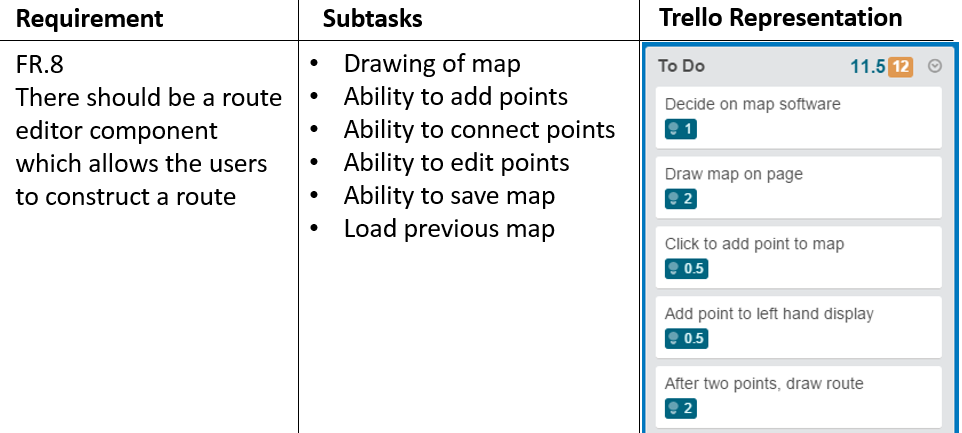
\includegraphics[width=0.8\textwidth]{images/implementation/task_breakdown.png}
	\end{center}
	\vspace{-6mm}
	\caption{Process for breaking down tasks, adding extra granularity with each step}
	\vspace{-10mm}	
\end{figure}
\ \\
\ \\
At the beginning of each week (where a week started on the day of project supervision meetings) the total list of tasks to be completed was evaluated. Based on priorities, prerequisites, and the Gantt chart produced for the project proposal (displayed in appendix \ref{sec:gantt}), a group of tasks would be selected for completion that week. Each task was given an estimated time of completion which would be used in conjunction with the number of work hours completed in the previous week to decide how many should be picked. This meant that a constant stream of work was completed every week, and that the project did not fall behind. Having weekly meetings was extremely useful, as they were a chance to course-correct if things weren't going to plan, to receive feedback on the progress of the project, and to get an outside perspective on how new features looked and behaved.

\newpage 
\subsection{Problems Encountered}
Assuming that a large project could be completed without any problems or issues along the way would be foolish, and this project was certainly no different. It is, therefore, extremely important to identify what these problems are, what the causes were, and how these can be prevented in the future. The biggest problem faced during the implementation of Niceway.to, was the lack of a proper testing framework. As new features were added, they were individually tested, and some minor integration testing was carried out with other parts of the system they may have an impact on. After this was done, the feature was assumed to be bug free, and progress on the project continued. However, on several occasions, a new feature would be added, tested briefly, and marked as complete, only to have it be the root cause of some problem further down the line, due to some unforeseen interaction with another component. This meant that a lot of time was dedicated to going back to previous features and fixing time, instead of pushing the project forward. The solution to this would be to implement unit testing on every aspect of the system. This would mean, after the addition of any features, a set of tests could be run to ensure that all components of the system are still functioning as expected. Considering how well integrated unit tests are with the Zend framework, their lack of inclusion is this project is even more worrying. The main reason for this is how some work on the project was prototyped before its official commencement. This prototyped code did not implemented testing, but was then directly included in the project. This meant that the speed of the initial stages of the project were accelerated, but meant that unit tests were left out, and with such a large code base now, it would troublesome to implement them at this point.\ \\
\ \\
The next major problem encountered was the lack of proper research into an adequate routing service. When implementing the functionality to draw a route between two points, not much research was conducted into which routing service would be the best, and instead the easiest to implement was selected. This initial routing service was the MapBox default routing service, which was extremely easy to implement, because MapBox was being used to provide the map. After implementing the functionality to draw these routes, it became apparently that the service had a limit to the number of points it could route at any one time (a maximum of twelve), and that the service was unreliable (at times it would be unable to provide any route at all). This meant that a new service needed to be selected (the Leaflet Routing Machine), and that a lot of the functionality for routing needed to be rewritten with this new library. This wasted a lot of time, as work that was previous deemed complete needed to be completed a second time. This could have been resolved by expanding the research conducted at the beginning of the project, and being more thorough in which software was investigated (instead of just back end and front end tools, it would have been beneficial to look at libraries that were required as well). \ \\
\ \\
The third major problem was lack of attention to detail in the creation of the requirements. At the beginning of the project, the client provided a specification for the project, which included all features he required. This was then converted into a requirements specification, with functional and non-functional requirements. However, during this conversion, some of the intricate details of the initial specification were lost which meant that, half way through the project, it was discovered that there was a large amount of functionality missing. Not only did this add extra pressure to the project, but also meant that many previous features had to be revisited and revised, which meant a lot of time had been wasted in the implementation procedure. In future, this can be avoided by paying much closer attention to the initial specification, and ensuring that all details are extracted as necessary, and getting the client to sign off on these extracted requirements.



